\chapter{自动加样系统硬件设计方案的确定}
自动加样控制系统包括一个控制器,有若干个功能模块。控制器为$AT89C52$单片机,功能模块为直角坐标系中三个方向的步进电机运动模块、三个位置传感器模块、加样机构的液位传感器模块和步进电机驱动模块、清洗模块等。三个步进电机运动模块在驱动模块的作用下实现了在三维空间内任意位置的定位,位置传感器使得检测机械臂复位情况以及防止机械臂在运动过程中发生干涉,液位传感器检测加样机构到达液面以下的位置
\section{控制器的选型}
本研究选用的控制器为$AT89C52$单片机,它是一款8位$CMOS$单片机,由美国公司$ATMEL$推出。$AT89C52$单片机嵌有$8K bytes$可反复擦写的闪存$ROM$存储器和$256$ $bytes$数据存储器;32个输入输出($I/O$)接口线,3个16位定时计数器,一个全双工串行通讯口,同时含有两个外中断口,共六个中断源;此外,片内配置振荡器和时钟电路。其空闲工作模式能保证$CPU$停止工作的同时其它模块如存储器、中断系统正常工作,掉电保护模式能及时保存$RAM$内容,使振荡器失去作用并其它部件工作直到接收到复位信号以保护系统\supercite{bib14}。$AT89C52$单片机强大的功能使其能够应用在较为复杂的控制系统中。该控制器的最小系统由复位电路和时钟电路组成,简单可靠。其电路图如\ref{fig:5-1}

\begin{figure}[htbp!]
	\centering
	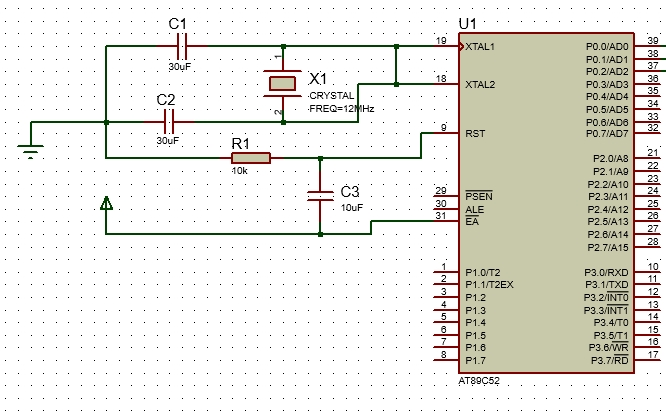
\includegraphics[height=7.5cm]{chap/figure/5-1.jpg}
	\caption{AT89C52最小系统简图}
	\label{fig:5-1}
\end{figure}

\section{步进电机的驱动电路}
一方面,$AT89C52$单片机的是输出功率非常小;另一方面,步进电机不能直接连接直流电源。因此,必须在步进电机和单片机之间接上驱动电路以保证前者的正常工作。步进电机的驱动器种类十分丰富,一般成熟步进电机产品都有配置的电机驱动器。在上一章节中我们选取了$Leetro$公司的DM5641E型号电机,那么步进电机的驱动器仍选取此公司配套的驱动器DMD605。该驱动器的脉冲响应频率最高可达360KHz,斩波频率为20KHz,最大驱动电流达5.6A/相,供电电压为+20VDC—+60VDC直流电源。其细分设定情况如表\ref{tab:5-1}。

\begin{table}[htbp]
	\centering
	\caption{DMD605细分设置}
	\begin{tabular}{cccccc}
		\toprule
		\toprule
		细分数  & 步数/转  &	SW5  & SW6  & SW7  & SW8 \\
		\midrule
		1  & 200  &  off  & off  & off  & off  \\
		2  & 400  & on  & on  & on  & on \\
		4  & 800  & on  & off & on  & on \\
		8  & 1600  & on  & off  & off  & on  \\
		\bottomrule
		\bottomrule
	\end{tabular}%
	\label{tab:5-1}%
\end{table}%

DMD605驱动器共有12个引脚,其接口引脚的解析情况如表\ref{tab:5-2}
\begin{table}[htbp]
	\centering
	\caption{DMD605引脚功能}
	\begin{tabular}{p{80pt}p{250pt}}
		\toprule
		\toprule
		引脚名称  & 功能 \\
		\midrule
		PUL+(+5V)、PUL-  & 脉冲信号:该引脚每接收到一个脉冲信号步进电机完成一次步进, 通过细分设置功能来设定每次的步进量;脉冲上升沿触发。 \\
		DIR+(+5V)、DIR- & 方向信号:该引脚通过电平的高低来更改电机转向, 实际转向还取决于电机绕组的联接情况;脉冲上升沿触发\\ 
		Ena+(+5V)、Ena-  & 使能信号:该引脚的功能为使能或禁止,导通时,驱动器将不再起向步进电机各相供电,使后者处于惯性状态。 \\
		\bottomrule
		\bottomrule
	\end{tabular}%
	\label{tab:5-2}%
\end{table}


在本设计中,在X、Y、Z三个加样运动方向上需要三个驱动器。通过对其引脚功能分析可知,每个DMD605驱动器占据单片机的三个输入输出端。以$X$方向为例,它分别占据单片机I/O口的P2.0、P2.1、P2.2。其中,I/O口P2.0接引脚PUL$-$控制步进电机的运动,I/O口P2.1连接引脚DIR$-$控制步进电机的转向,I/O口P1.3控制使能信号。其它两个方向同理,其中$Y$方向驱动器的三个引脚分别对应连接I/O口P2.3、P2.4、P2.4;$Z$方向的驱动器三个引脚对应连接P0口的I/O口P0.0、P0.1、P0.2,但是P0口用作普通输入输出端口时,输出电路为漏极开路电路,需要接上拉电阻\supercite{bib15}。$AT89C52$控制器与X(Y)方向平动步进电机驱动器的电路连线图如图\ref{fig:5-2},Z方向升降步进电机驱动器与$AT89C52$单片机电路连接图如\ref{fig:5-3}
\begin{figure}[htbp!]
	\centering
	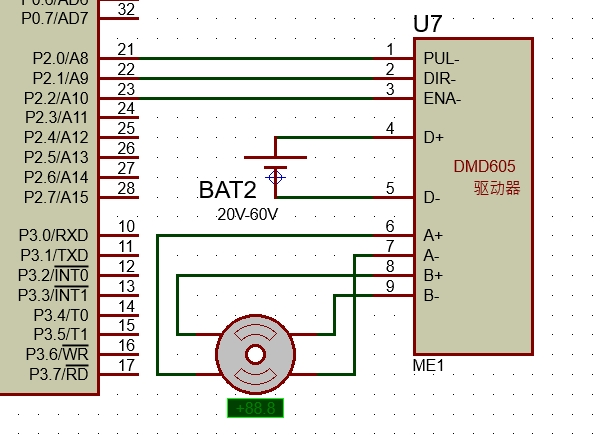
\includegraphics[height=8.0cm]{chap/figure/6-3.jpg}
	\caption{X(Y)方向驱动器的电路连线图}
	\label{fig:5-2}
\end{figure}

\begin{figure}[htbp!]
	\centering
	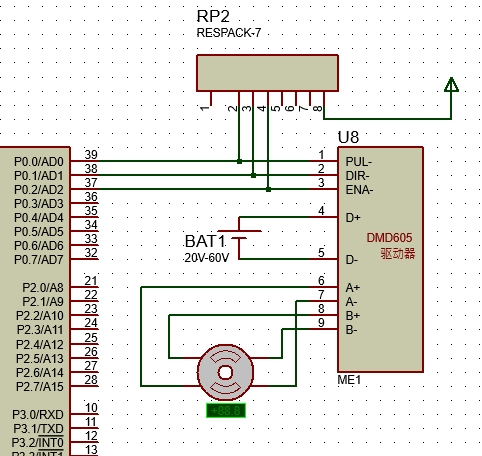
\includegraphics[height=9.8cm]{chap/figure/6-4.jpg}
	\caption{Z方向驱动器的电路连线图}
	\label{fig:5-3}
\end{figure}

\section{液位检测模块电路}
自动加样过程中,加样针逐渐靠近液面,当加样针针头顶部到达液面以下某一位置时,要求驱动加样针的步进电机停止工作,以进行取样和释样,从而最大可能避免试液之间的交叉污染和加样误差的发生。这就要求加样机构能快速检测到液面位置,并及时作出反馈,从而进行下一步动作。本部分将对液位检测模块的电路进行设计。

根据上文4.5节,我们设计了一种电容式液位传感器。它利用加样针的内壁和外壁作为电容场的两个极板,通过两极板之间介质的介电常数突变原理来捕获液位位置。电容式传感器可以将电容变化的模拟量转变成某种中间物理量,再通过硬件电路将中间物理量转置成数字信号输出。不同的电容式液位检测装置将电容变化量转置的中间量也不尽相同,如基于电容-相位变化原理\supercite{bib17}、基于电容-幅度变化原理、基于电容-谐振原理等\supercite{bib18}。

本研究采用基于电容-频率激变原理\supercite{bib16},设计一种液面检测电路图。电容-频率激变原理通俗地讲,就是将电容值的跃变转化成中间量脉冲信号频率的激变进而输出,本研究液面检测模块电路图如\ref{fig:5-4}。

\begin{figure}[htbp!]
	\centering
	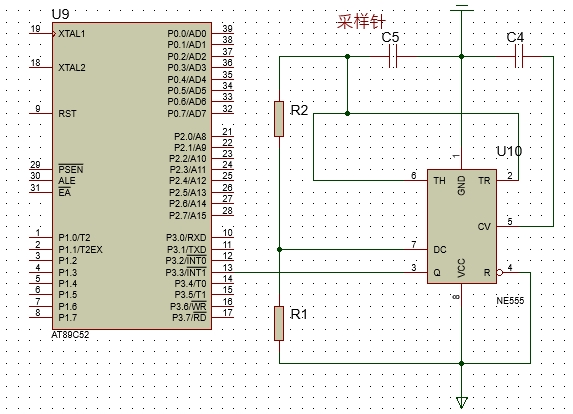
\includegraphics[height=9.8cm]{chap/figure/5-6.jpg}
	\caption{液面检测模块电路图}
	\label{fig:5-4}
\end{figure}

如图5-4所示,该电路的核心是多谐振荡电路,它由电容C4、C5,电阻R1、R2和555定时器组成的,555定时器的输出引脚3连接单片机的中断源引脚P3.3,放电引脚7连接电阻R1、R2,电阻R1的另一端、重置引脚4和接电引脚8共同接电源,电阻R2的另一端、重置锁定引脚和放电引脚共同接C5采样针的内壁,C5采样针的外壁、电容C4和接地引脚共同接地。

加样针的内、外壁可以代替振荡电路中的电容C5。加样针为到达液面之前,多谐振荡电路中的电容C1处在正常工作状态,能进行正常的充放电,此时振荡电路产生周期性脉冲信号,其周期为T且有:

$$T = {T_1} + {T_2} \eqno{(5-1)}$$
$${T_1} = \left( {{R_1} + {R_2}} \right) \times C \times \ln 2 \eqno{(5-2)} $$
$${T_2} = {R_2} \times C \times \ln 2 \eqno{(5-3)}$$

式(5-1)中${T_1}$、${T_2}$分别为电容C5的充电、放电时间,综合式(5-2)、(5-3)可得:
$$T = \ln 2\left( {{R_1} + 2{R_2}} \right)C \eqno{(5-4)}$$

加样针进入液面之后,试液连接加样针的内外壁导致C5短路,即C为0,由式(5-4)知T等于0,此时脉冲方波消失而产生定值波。单片机每隔一小段时间就监测INT1是否接收到下降沿信号,然后通过计数器a累加计数。当计数器a中的值超过2时将a置零重新计数,说明此时谐波振荡电路产生周期性脉,加样针为到达液面;当a小于2时,说明谐波振荡电路产生定值波,说明加样针已到达液面。此时,单片机控制$Z$轴步进电机继续以一定速度驱动加样针下降至液面下$1-2mm$后停止,进行取样或释样动作。












